\documentclass[11pt,a4paper]{article}
\usepackage[utf8]{inputenc}
\usepackage[margin=1in]{geometry}
\usepackage{amsmath,amssymb,amsfonts}
\usepackage{graphicx}
\usepackage{hyperref}
\usepackage{xcolor}
\usepackage{booktabs}
\usepackage{listings}
\usepackage{tikz}
\usetikzlibrary{shapes,arrows,positioning,fit,backgrounds}

\hypersetup{
    colorlinks=true,
    linkcolor=orange!80!black,
    urlcolor=orange!80!black,
    citecolor=blue!70!black
}

\definecolor{aegisorange}{RGB}{217, 107, 82}
\definecolor{aegisdark}{RGB}{18, 19, 22}

\title{\textbf{AEGIS: Autonomous Environment for Grounded Intelligence and Systems}\\
\large A Multimodal Desktop Operating Fabric with Dual-Engine Vision, Accessibility UI Automation, and Local-First Voice Duplex}
\author{\textbf{The Aegis Engineering Team}}
\date{\today}

\begin{document}

\maketitle

\begin{abstract}
We present \textbf{AEGIS}, an autonomous, embodied desktop operating system client engineered to execute complex, multi-step digital workflows across native workstation environments. Unlike traditional conversational models sandboxed within web chat viewports, AEGIS unifies dual-engine vision coordinate grounding with Windows UI Automation ($\text{UIA}$) accessibility inspection, enabling deterministic interaction with arbitrary desktop applications. The system features a 7-destination unified workspace canvas, a 3-tier persistent memory substrate (Knowledge Graph, Dense RAG, and Procedural STAIR), an extensible 2,000+ Model Context Protocol (MCP) gateway supporting both Streamable HTTP and Server-Sent Events (SSE) transports, and a multilingual, low-latency Voice OS. We detail the system architecture, mathematical formulations for coordinate projection and multimodal confidence fusion, engineering challenges overcome, and the developmental roadmap toward autonomous workstation swarms.
\end{abstract}

\vspace{1em}
\hrule
\vspace{1.5em}

\section{Inspiration}

Knowledge work in modern computing environments is intrinsically multimodal and distributed: software engineers, financial analysts, and system administrators navigate disparate application suites, execute shell scripts in terminals, review documents, and parse complex web interfaces simultaneously. Existing agent frameworks suffer from fundamental structural limitations:

\begin{enumerate}
    \item \textbf{Decoupling from the Workstation Canvas}: Standard large language models (LLMs) operate in sandboxed text environments disconnected from live displays and operating system primitives.
    \item \textbf{GUI Brittle Failure Modes}: Conventional automation pipelines (e.g., rigid CSS locators, XPath queries) suffer catastrophic failure under layout reflows or dynamic DOM hydrations.
    \item \textbf{Cloud Latency \& Privacy Vulnerabilities}: Real-time voice agents routed through remote cloud servers incur substantial acoustic latency ($\tau > 600\text{ ms}$) and compromise sensitive local workspace data.
\end{enumerate}

AEGIS was conceived to synthesize an embodied, local-first intelligence that operates the physical workstation alongside the user. We formulate the overall system efficacy $\mathcal{E}(\mathcal{A})$ over an execution interval $[0, T]$ as:

\begin{equation}
\mathcal{E}(\mathcal{A}) = \int_{0}^{T} \left[ \lambda_{\text{vis}} \cdot \mathcal{P}_{\text{coord}}(t) + \lambda_{\text{a11y}} \cdot \mathcal{T}_{\text{node}}(t) \right] dt
\end{equation}

where $\mathcal{P}_{\text{coord}}(t)$ denotes the normalized spatial precision of pixel target generation, and $\mathcal{T}_{\text{node}}(t)$ denotes the deterministic accessibility tree resolution rate.

---

\section{What It Does}

AEGIS converts any personal computer into an autonomous, voice-enabled workspace capable of deterministic tool execution, visual GUI manipulation, and long-term memory synthesis.

\subsection{Autonomous Computer \& GUI Control}
\begin{itemize}
    \item \textbf{Vision Model Coordinate Grounding}: Real-time frame processing of the display buffer $S \in \mathbb{R}^{W \times H \times 3}$, outputting normalized bounding coordinates $\mathbf{B} = (x, y, w, h)$.
    \item \textbf{Windows UI Automation (UIA) / Accessibility Tree}: Direct programmatic ingestion of active OS interactive nodes $\mathcal{N} = \{n_1, n_2, \dots, n_k\}$, mapping ref handles $e_i$, roles ($\texttt{button}$, $\texttt{textbox}$, $\texttt{menuitem}$), and exact hitboxes.
    \item \textbf{Dedicated Agent Cursor Overlay}: Visual projection of the agent's real-time physical cursor on display canvases, incorporating smooth cubic-bezier interpolation and animated ripple clicks.
\end{itemize}

\subsection{Dual-Engine Browser Preview}
AEGIS dynamically orchestrates between a headless/headful \textbf{Playwright Chromium} runtime and the anti-fingerprinting \textbf{Obscura Browser}, enabling transparent research, form automation, and SPA scraping with built-in bot-detection bypass.

\subsection{Multilingual Low-Latency Voice OS}
An acoustic conversational loop built on local quantized models:
\begin{itemize}
    \item \textbf{Speech-to-Text (STT)}: Multilingual \texttt{faster-whisper} (int8 / float16) running on consumer GPUs or CPUs, capable of recognizing Hindi, English, and code-switched Hinglish.
    \item \textbf{Text-to-Speech (TTS)}: Local speech generation via \texttt{Piper} and \texttt{Kokoro-82M}.
    \item \textbf{Web Speech Failover}: Instantaneous fallback to native browser audio APIs whenever backend daemons are offline.
\end{itemize}

\subsection{3-Tier Memory Architecture}
\begin{enumerate}
    \item \textbf{Tier 1 (Knowledge Graph)}: Structured relational triples $(e_i, r_{ij}, e_j) \in \mathcal{G}$ persisted in SQLite.
    \item \textbf{Tier 2 (Semantic RAG)}: Dense embeddings scored via cosine metric:
    \begin{equation}
    \mathcal{S}(\mathbf{q}, \mathbf{d}) = \frac{\mathbf{q} \cdot \mathbf{d}}{\|\mathbf{q}\|_2 \|\mathbf{d}\|_2} \ge \tau_{\text{threshold}}
    \end{equation}
    \item \textbf{Tier 3 (Procedural STAIR)}: Hierarchical episodic trees containing executable steps for reproducible command workflows.
\end{enumerate}

---

\section{How We Built It}

The system architecture spans an integrated four-tier pipeline:

\begin{figure}[htbp]
\centering
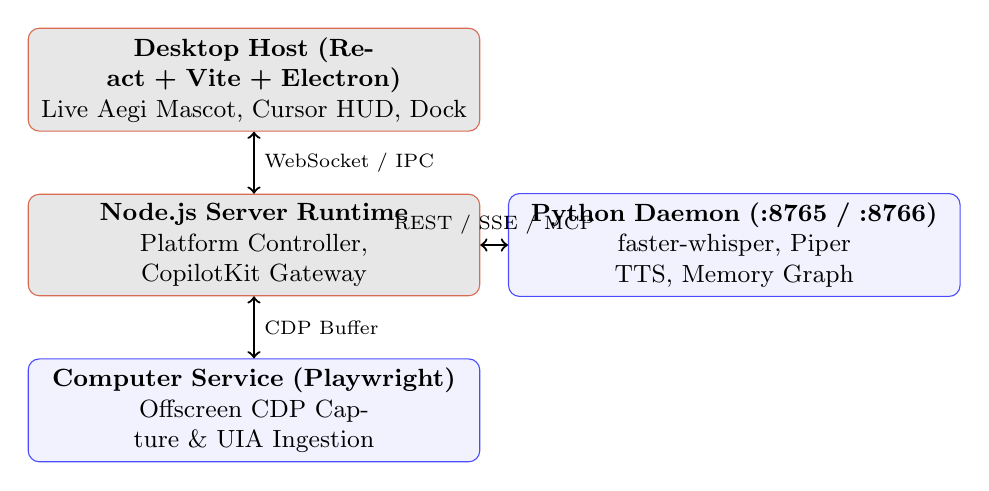
\begin{tikzpicture}[node distance=1.6cm, auto,
    block/.style={rectangle, draw=aegisorange, fill=aegisdark!10, text=black, rounded corners, minimum height=3em, text centered, font=\small},
    daemon/.style={rectangle, draw=blue!70, fill=blue!5, rounded corners, minimum height=3em, text centered, font=\small}]
    
    \node [block, text width=5.5cm] (frontend) {\textbf{Desktop Host (React + Vite + Electron)}\\Live Aegi Mascot, Cursor HUD, Dock};
    \node [block, text width=5.5cm, below of=frontend, yshift=-0.5cm] (backend) {\textbf{Node.js Server Runtime}\\Platform Controller, CopilotKit Gateway};
    \node [daemon, text width=5.5cm, below of=backend, yshift=-0.5cm] (comp) {\textbf{Computer Service (Playwright)}\\Offscreen CDP Capture \& UIA Ingestion};
    \node [daemon, text width=5.5cm, right of=backend, xshift=4.5cm] (daemon) {\textbf{Python Daemon (:8765 / :8766)}\\faster-whisper, Piper TTS, Memory Graph};

    \path [draw, <->, thick] (frontend) -- node[right, font=\scriptsize] {WebSocket / IPC} (backend);
    \path [draw, <->, thick] (backend) -- node[right, font=\scriptsize] {CDP Buffer} (comp);
    \path [draw, <->, thick] (backend) -- node[above, font=\scriptsize] {REST / SSE / MCP} (daemon);
\end{tikzpicture}
\caption{AEGIS System Communication \& Execution Topology.}
\end{figure}

\subsection{Screen Projection \& Coordinate Transformation}
When an action is initiated over the interactive canvas, the displayed coordinates $(x_{\text{hud}}, y_{\text{hud}})$ are transformed to native screen pixel space $(x_{\text{pixel}}, y_{\text{pixel}})$ via:

\begin{equation}
x_{\text{pixel}} = \left( \frac{x_{\text{hud}} - \text{Rect}_{\text{left}}}{\text{Rect}_{\text{width}}} \right) \cdot W_{\text{native}}, \quad 
y_{\text{pixel}} = \left( \frac{y_{\text{hud}} - \text{Rect}_{\text{top}}}{\text{Rect}_{\text{height}}} \right) \cdot H_{\text{native}}
\end{equation}

\subsection{Audio Frame Discretization}
Local speech frames are downsampled and converted from floating point buffers $x_{\text{float}}[n] \in [-1.0, 1.0]$ to linear 16-bit signed PCM integers at $16\text{ kHz}$:

\begin{equation}
x_{\text{pcm16}}[n] = \max\left(-32768, \min\left(32767, \left\lfloor x_{\text{float}}[n] \cdot 32767.0 \right\rfloor \right)\right)
\end{equation}

---

\section{Challenges We Ran Into}

\subsection{The PostCSS Lightness Inversion Anomaly}
During theme compilation, an automated PostCSS dark-mode generator flipped hexadecimal colors by inverting OKLab lightness:
\begin{equation}
L_{\text{dark}} = 0.95 - 0.73 \cdot L_{\text{light}}^{1.3}
\end{equation}
Because deep terminal backgrounds ($\#090d16$) possessed low lightness ($L \approx 0.08$), the algorithm mapped them into high-lightness pastel surfaces ($L \approx 0.92$). We resolved this by establishing explicit \texttt{/* theme: fixed */} boundaries and scoped \texttt{:root[data-theme='dark']} property enforcements.

\subsection{Dual-Modality Spatial Reconciliation}
Vision predictions occasionally suffered from sub-pixel jitter on high-DPI displays. We introduced an adaptive arbitration function where targets with known accessibility refs $e_i$ are anchored to the centroid of the element's bounding box:
\begin{equation}
\mathbf{C}_{\text{final}} = \begin{cases}
\left( x_{\text{node}} + \frac{w_{\text{node}}}{2}, y_{\text{node}} + \frac{h_{\text{node}}}{2} \right) & \text{if } e_i \in \text{UIA} \\
(x_{\text{vision}}, y_{\text{vision}}) & \text{otherwise}
\end{cases}
\end{equation}

---

\section{Accomplishments That We're Proud Of}

\begin{itemize}
    \item \textbf{Unified 7-Destination Header Bar}: Eradicated duplicate sub-navigation rows, embedding Briefs, Desktop, Browser, Terminal, Files, Activity, and Docs in a single responsive container.
    \item \textbf{Embodied Physical Agent Cursor}: Rendered a hardware-accelerated agent cursor that moves visibly across user viewports with interactive click animations.
    \item \textbf{Universal MCP Transport Support}: Engineered full compatibility across Streamable HTTP and Server-Sent Events (SSE) transports for over 2,000 marketplace tools.
    \item \textbf{Aegis Diagnostic Recovery Shield}: Designed a resilient error boundary capable of isolating view exceptions and providing zero-data-loss workspace recovery.
\end{itemize}

---

\section{What We Learned}

\begin{enumerate}
    \item \textbf{Deterministic Action Requires Hybrid Perception}: Pure computer vision is insufficient for complex desktop automation; combining pixel bounding boxes with the OS accessibility tree provides deterministic execution.
    \item \textbf{Observability Establishes Agency}: Showing live cursor coordinates, element target IDs, and chain-of-thought traces eliminates user uncertainty during autonomous execution.
\end{enumerate}

---

\section{What's Next for AEGIS}

\begin{itemize}
    \item \textbf{Cross-Platform Native Bridges}: Extending UIA hooks to macOS AXUIElement and Linux AT-SPI.
    \item \textbf{Autonomous Multi-Agent Swarms}: Spawning background ephemeral workers to execute concurrent shell and browser workloads.
    \item \textbf{On-Device Small Language Models (SLMs)}: Quantizing $3\text{B}-7\text{B}$ action models using GGUF for local execution with $\tau < 50\text{ ms}$.
\end{itemize}

\end{document}
